\documentclass[11pt]{article}

% ============================================================
% COMPILATION
% ============================================================
%
% Required compiler: XeLaTeX
%
% Recommended build sequence:
% XeLaTeX -> Biber -> XeLaTeX -> XeLaTeX
%

% ============================================================
% DOCUMENT EDITION
% ============================================================

\newif\iftutornotes

\tutornotestrue       % TA / Tutor edition
% \tutornotesfalse    % Student edition

% ============================================================
% PACKAGES
% ============================================================

\usepackage[a4paper,margin=1in]{geometry}

% XeLaTeX font system
\usepackage{fontspec}
\usepackage{unicode-math}

\setmainfont{TeX Gyre Termes}
\setsansfont{TeX Gyre Heros}
\setmonofont{Latin Modern Mono}
\setmathfont{TeX Gyre Termes Math}

\usepackage{microtype}
\usepackage{enumitem}
\usepackage{booktabs}
\usepackage{array}
\usepackage{longtable}
\usepackage{xcolor}
\usepackage{hyperref}
\usepackage{listings}
\usepackage{tcolorbox}
\usepackage{titlesec}
\usepackage{fancyhdr}
\usepackage[backend=biber,style=ieee]{biblatex}

% ============================================================
% DOCUMENT METADATA
% ============================================================

\newcommand{\CourseTitle}{Physical AI, TAICA}
\newcommand{\InstructorName}{Human-centered Intelligent System Lab}
\newcommand{\InstructorEmail}{National Yang Ming Chiao Tung University}

\newcommand{\AssignmentTitle}{Homework 1: 3D Scene Reconstruction}
\newcommand{\Semester}{Fall 2026}

% ============================================================
% BIBLIOGRAPHY
% ============================================================

\addbibresource{refs.bib}

% ============================================================
% TABLE SETTINGS
% ============================================================

\newcolumntype{L}[1]{>{\raggedright\arraybackslash}p{#1}}

% ============================================================
% HYPERLINK SETTINGS
% ============================================================

\hypersetup{
    colorlinks=true,
    linkcolor=blue!50!black,
    citecolor=blue!50!black,
    urlcolor=blue!50!black
}

% ============================================================
% PAGE STYLE
% ============================================================

\setlength{\headheight}{14pt}

\pagestyle{fancy}
\fancyhf{}

\lhead{\CourseTitle}
\rhead{\AssignmentTitle}
\cfoot{\thepage}

% ============================================================
% LIST SETTINGS
% ============================================================

\setlist[itemize]{
    topsep=3pt,
    itemsep=2pt,
    parsep=0pt,
    leftmargin=1.5em
}

\setlist[enumerate]{
    topsep=3pt,
    itemsep=2pt,
    parsep=0pt,
    leftmargin=1.6em
}

% ============================================================
% COLORS
% ============================================================

\definecolor{codebg}{RGB}{248,248,248}
\definecolor{commentgreen}{RGB}{0,110,60}
\definecolor{keywordblue}{RGB}{20,70,150}

% A single restrained color for all internal teaching notes.
\definecolor{tutorblue}{RGB}{65,88,110}
\definecolor{tutorbg}{RGB}{247,249,251}

% ============================================================
% TA / TUTOR NOTE SYSTEM
% ============================================================

% All material intended only for teaching staff must use this
% environment. Do not use separate teacher/grading/TA colors.
%
% In student mode, the complete environment body disappears.

\NewDocumentEnvironment{tutornote}{+b}
{%
    \iftutornotes
        \begin{tcolorbox}[
            colback=tutorbg,
            colframe=tutorblue,
            boxrule=0.4pt,
            arc=1mm,
            left=7pt,
            right=7pt,
            top=6pt,
            bottom=6pt,
            before skip=8pt,
            after skip=8pt
        ]
        {\small
        \color{tutorblue}
        \textbf{TA/Tutor Note.}\par
        \medskip
        #1}
        \end{tcolorbox}
    \fi
}
{}

% Optional edition indicator.
% It appears only in the teaching edition.

\newcommand{\EditionLabel}{%
    \iftutornotes
        \begin{center}
            {\small\color{tutorblue}
            TA / Tutor Teaching Edition}
        \end{center}
        \vspace{0.5em}
    \fi
}

% ============================================================
% LISTINGS
% ============================================================

\lstdefinelanguage{turtle}{
    alsoletter={:@},
    morekeywords={
        @prefix,
        a,
        owl:,
        rdf:,
        rdfs:,
        xsd:
    },
    sensitive=true,
    morecomment=[l]{\#},
    morestring=[b]"
}

\lstset{
    basicstyle=\ttfamily\small,
    backgroundcolor=\color{codebg},
    breaklines=true,
    frame=single,
    framerule=0.2pt,
    rulecolor=\color{black!20},
    keywordstyle=\color{keywordblue}\bfseries,
    commentstyle=\color{commentgreen},
    stringstyle=\color{black!70},
    columns=fullflexible,
    keepspaces=true,
    showstringspaces=false
}

\lstdefinestyle{codesnippet}{
    numbers=none,
    aboveskip=0.75\baselineskip,
    belowskip=0.85\baselineskip,
    frame=single,
    framerule=0.2pt,
    rulecolor=\color{black!20},
    backgroundcolor=\color{codebg},
    basicstyle=\ttfamily\small,
    breaklines=true,
    columns=fullflexible,
    keepspaces=true,
    showstringspaces=false
}

\newcommand{\code}[1]{\texttt{\detokenize{#1}}}

% ============================================================
% TITLE
% ============================================================

\title{\textbf{\AssignmentTitle}}
\author{
    \InstructorName\\
    \InstructorEmail
}
\date{\Semester}

% ============================================================
% DOCUMENT
% ============================================================

\begin{document}
\maketitle
\EditionLabel

% ============================================================
\section{Introduction}
% ============================================================
Imagine asking a household robot to bring you something from the kitchen. To do that safely, it needs a useful picture of the home: where rooms and furniture are, how spaces connect, and where it can move without collisions. A 3D scene map gives the robot this spatial understanding and can support navigation, object finding, and assistance \cite{szeliski2022computer,replica2019}.

In this assignment, you will reconstruct apartment\_0, an indoor scene from the Replica dataset \cite{replica2019}, from red-green-blue and depth (RGB-D) observations. You will transform depth images into 3D point clouds, align observations from different viewpoints, combine them into a scene, and evaluate the resulting map and camera trajectory. These are the same kinds of steps a robot uses to turn sensor data into a representation it can act on \cite{hartley2004multiple,chen1992object}.

This is an enhanced version of the standard 3D reconstruction task: in addition to implementing the required Open3D pipeline, you will verify the input data and use measurements to explain how capture conditions affect reconstruction. Missing or noisy depth, insufficient viewpoint overlap, and large frame-to-frame motion can all make alignment difficult \cite{shin2019camera,immerkaer1996fast}.

The assignment has two phases. Phase 1 uses a provided first-floor capture. Phase 2 uses the Habitat simulator (Habitat-Sim) to collect a second-floor capture yourself. Both phases use the same reconstruction and verification workflow, so you can compare a supplied capture with one shaped by your own navigation and collection choices \cite{replica2019,habitatsim2020}.

% ============================================================
\section{Learning Objectives}
% ============================================================
By completing this assignment, you will be able to:
\begin{enumerate}
\item Understand the pipeline from visual perception to 3D scene reconstruction, including observation collection, geometric representation, alignment, mapping, and evaluation \cite{szeliski2022computer,replica2019}.
\item Understand how the pinhole camera model and depth measurements determine the geometry of a reconstructed scene \cite{hartley2004multiple}.
\item Understand how global and local registration choices affect the stability, quality, and computational cost of scene reconstruction \cite{fischler1981ransac,chen1992object,open3dglobal}.
\item Understand the importance of data quality and its impact on 3D reconstruction by relating observable image and depth conditions to alignment behavior \cite{shin2019camera,immerkaer1996fast}.
\item Evaluate and communicate reconstruction quality using reproducible experiments, visual evidence, and the required Mean L2 Distance metric.
\end{enumerate}

% ============================================================
\section{Assignment Overview}
% ============================================================
\subsection{RGB-D Scene Reconstruction}
The reconstruction pipeline loads synchronized RGB-D observations and ground-truth (GT) camera poses.

Each RGB-D frame contains a color image and a depth image captured from one camera pose.

Given calibrated intrinsics $(f_x,f_y,c_x,c_y)$, a valid depth sample $Z=D(u,v)/s$ at pixel $(u,v)$ back-projects to camera coordinates:
\[
X=\frac{(u-c_x)Z}{f_x},\qquad Y=\frac{(v-c_y)Z}{f_y},\qquad Z=\frac{D(u,v)}{s},
\]
The symbols in this equation are annotated as follows:
\[
\begin{aligned}
X,Y,Z &:\ \text{camera-coordinate components}, & u,v &:\ \text{pixel column and row},\\
f_x,f_y &:\ \text{horizontal and vertical focal lengths (pixels)}, & c_x,c_y &:\ \text{principal-point coordinates (pixels)},\\
D(u,v) &:\ \text{raw depth value}, & s &:\ \text{raw-to-metric depth scale}.
\end{aligned}
\]
Repeating this operation forms a point cloud. The required pipeline downsamples point clouds, estimates an initial transform with Random Sample Consensus (RANSAC) for global registration, and refines it with Iterative Closest Point (ICP) for local registration \cite{hartley2004multiple,fischler1981ransac,chen1992object,open3dglobal}.

The estimated transforms place aligned clouds in a shared coordinate system, where they are accumulated into a 3D scene map. The pipeline also composes an estimated camera trajectory, visualizes the map and trajectories, and evaluates the result against GT poses when available. The estimated trajectory must be shown in red and the GT trajectory in black; remove the ceiling from the scene visualization when it obstructs inspection \cite{replica2019}.

\paragraph{Required evaluation metric.}
The required metric is the \textbf{Mean L2 Distance}, the mean Euclidean $L_2$ distance between estimated and GT camera positions. For $N$ evaluated frames, use
\[
\operatorname{MeanL2}=\frac{1}{N}\sum_{i=1}^{N}\left\|\hat{\mathbf p}_i-\mathbf p_i^{\mathrm{GT}}\right\|_2,
\]
The symbols in this equation are annotated as follows:
\[
\begin{aligned}
N &:\ \text{number of evaluated frames}, & i &:\ \text{frame index},\\
\hat{\mathbf p}_i=(\hat{x}_i,\hat{y}_i,\hat{z}_i) &:\ \text{estimated camera position},\\
\mathbf p_i^{\mathrm{GT}}=(x_i^{\mathrm{GT}},y_i^{\mathrm{GT}},z_i^{\mathrm{GT}}) &:\ \text{ground-truth camera position},\\
\|\cdot\|_2 &:\ \text{Euclidean }L_2\text{ norm}.
\end{aligned}
\]
All position coordinates are expressed in the shared scene coordinate system.
You \textbf{MUST} report this Mean L2 Distance in the report for every reconstruction being compared. Do not replace it with root mean square error, mean absolute error, or a metric based on an additional fitted alignment. Report the evaluated frame count, unit, runtime, and relevant parameters together with the metric.

The two phases apply this same pipeline to different floors of apartment\_0. Phase 1 uses the provided first-floor RGB-D data; Phase 2 uses second-floor RGB-D observations collected by students with a Habitat-Sim agent. Compare viewpoint coverage, frame spacing, overlap, registration choices, visual map quality, Mean L2 Distance, and runtime across the two reconstructions \cite{habitatsim2020}.

\subsection{Data Verification}
Reconstruction can fail for several reasons, and no single scalar predicts success. Students MUST inspect and examine the RGB-D inputs directly, including representative RGB and depth images, metadata, missing or invalid depth, and frame-to-frame changes. These diagnostic measurements describe one RGB image, one depth image, or a consecutive depth pair. They support input inspection and interpretation of alignment behavior; they do not replace reconstruction or prove causation. RGB exposure factors provide context about appearance and feature visibility; the geometric ICP step aligns depth-derived point clouds \cite{shin2019camera,chen1992object}.

{\renewcommand{\arraystretch}{1.28}
\begin{longtable}{>{\centering\arraybackslash}p{0.16\linewidth} L{0.14\linewidth} L{0.32\linewidth} L{0.21\linewidth}}
\toprule
\textbf{Factor} & \textbf{Scope} & \textbf{Definition and use} & \textbf{Reconstruction relation} \\
\midrule
\endhead
\parbox[t]{\linewidth}{\centering\texttt{Highlight}\\\texttt{Clipping}} & RGB image & Fraction of pixels whose maximum color channel meets an explicitly chosen high threshold. & Records overexposure; contextual for depth-only ICP. \cite{shin2019camera} \\
\parbox[t]{\linewidth}{\centering\texttt{Shadow}\\\texttt{Clipping}} & RGB image & Fraction of pixels for which all color channels meet an explicitly chosen low threshold. & Records underexposure; contextual for appearance and feature visibility. \cite{shin2019camera} \\
\parbox[t]{\linewidth}{\centering\texttt{High}\\\texttt{Frequency}\\\texttt{Depth}\\\texttt{Residual}} & Depth image & Robust estimate of high-frequency depth noise using a 3-by-3 high-pass response and median absolute deviation scaling. & Noisy surfaces may perturb back-projected points and local alignment. \cite{immerkaer1996fast} \\
\parbox[t]{\linewidth}{\centering\texttt{Flying}\\\texttt{Pixel}\\\texttt{Ratio}} & Depth image & Fraction of mixed-boundary returns identified from local depth neighborhoods and plane support. & Inconsistent boundary points may affect geometric alignment. \\
\parbox[t]{\linewidth}{\centering\texttt{Valid}\\\texttt{Tile}\\\texttt{Coverage}} & Depth image & Fraction of fixed-size tiles whose valid-depth share reaches a documented support level. & Describes spatial distribution of usable geometry. \\
\parbox[t]{\linewidth}{\centering\texttt{Identity}\\\texttt{Median}\\\texttt{Depth}\\\texttt{Change}} & Depth pair & Median absolute depth change at corresponding pixel coordinates over jointly valid samples. & Coarse motion/change indicator; large change can signal weaker pairwise alignment. \\
\parbox[t]{\linewidth}{\centering\texttt{Joint}\\\texttt{Valid}\\\texttt{Depth}\\\texttt{Ratio}} & Depth pair & Fraction of pixel coordinates with valid depth in both images. & Proxy for shared support; geometry and correspondence quality also matter. \\
\parbox[t]{\linewidth}{\centering\texttt{Prior}\\\texttt{Warp}\\\texttt{Depth}\\\texttt{Residual}} & Depth pair & Median geometric depth residual after warping one frame under a motion prior. & Indicates disagreement with predicted alignment; depends on prior and visibility. \\
\bottomrule
\end{longtable}
}

Each factor definition specifies its input scope, observable, units or range, measurement parameters, and limitations. A single-image factor links to its RGBImage or DepthImage; a pair factor links to the two ordered observations used. Measurements remain numeric observations with settings and provenance.

\subsection{Vocabulary for Data Verification}
The reconstruction pipeline above turns a sequence of observations into a map, but interpreting that map depends on knowing which observations produced it. This is especially useful when comparing the supplied first-floor capture in Phase 1 with the second-floor capture students collect in Phase 2: a map artifact or alignment failure should be traceable to the frames and conditions that may have contributed to it. The labels below give the assignment tools a shared vocabulary for organizing that evidence. Use them to inspect and explain the data; you do not need to implement a separate data-management system.

\subsubsection{Basic Building Blocks}
\begin{itemize}
\item \textbf{Batch}: One capture directory and its shared camera information.
\item \textbf{Frame}: One indexed observation, with its RGB image, depth image, and camera pose when available.
\item \textbf{RGBImage}: The color image for a frame.
\item \textbf{DepthImage}: The depth image for the same frame, with its depth scale and invalid-value convention.
\item \textbf{RGBPair}: Two ordered RGB images that can be inspected together.
\item \textbf{DepthPair}: Two ordered depth images used for pair-level checks and alignment.
\item \textbf{Experiment}: One named reconstruction attempt on a batch.
\item \textbf{FactorMeasurement}: A numeric observation linked to the factor and image or frame pair it describes.
\item \textbf{Single-image factor}: A measurement made from one RGBImage or DepthImage.
\item \textbf{Depth-pair factor}: A measurement made from two depth observations.
\end{itemize}

During each phase, connect measurements to the observations they describe and to the reconstruction experiment that used them. A single-image measurement points to one RGB or depth image; a depth-pair measurement points to the ordered frames used for that check. If a pair measurement is unusual, inspect both frames and their alignment, then consider whether it helps explain an artifact in the map or a change in the estimated trajectory. Record the value, settings, and source links so the two phases and any additional runs can be compared. These measurements are evidence for interpreting reconstruction results, not standalone verdicts about whether a capture or alignment succeeded \cite{chen1992object}.

% ============================================================
\section{Environment Setup and Preparation}
% ============================================================
\subsection{Pixi installation}
Pixi manages the repository's pinned software environment. Install it using the official instructions for your operating system, then restart the shell so its executable is available on the system path \cite{pixiinstall}.
\begin{lstlisting}[language=bash]
curl -fsSL https://pixi.sh/install.sh | sh
# Or use the official package-manager instructions for your platform.
\end{lstlisting}

\subsection{Repository installation}
The main support target is 64-bit Linux. Habitat-Sim and the course workflow are configured and verified primarily on Linux. macOS and Windows with WSL may be used for development, but platform-specific graphics or binary differences may require adjustments \cite{habitatsiminstall}.

\subsubsection{Linux}
Clone the course repository and install its Habitat environment from the repository root:
\begin{lstlisting}[language=bash]
git clone --recurse-submodules https://github.com/HCIS-Lab/physicalai26-hw.git
cd physicalai26-hw/hw1
pixi install -e habitat
pixi run -e habitat python -c "import open3d, rdflib; print('ready')"
\end{lstlisting}

\subsubsection{macOS}
Install Pixi with the macOS method in its official guide. Clone the repository as above and attempt \code{pixi install -e habitat}. Linux remains the primary support target; if simulator binaries or visualization dependencies are unavailable, use Linux or WSL \cite{pixiinstall,habitatsiminstall}.

\subsubsection{Windows with WSL}
Install WSL2 with Ubuntu, then run Linux commands inside the WSL terminal. Keep the repository and datasets within the WSL Linux filesystem. Native Windows is not the main supported target \cite{microsoftwsl}.

\subsection{Data and Collection Resources}
The repository root is the directory containing \code{pixi.toml}; the assignment code is under \code{hw1/}. Both phases use a capture directory with one RGB image and one depth image per frame. The filename stem identifies the frame, so matching stems MUST be preserved.

\subsubsection{Phase 1: Provided Dataset}
The first-floor capture is provided to students through the course system. Unpack it directly under the repository's \code{eval/} directory. Use the capture directory name supplied with the course materials:
\begin{lstlisting}
<repository-root>/eval/<phase1-capture-dir>/
\end{lstlisting}
Do not add another nested directory or rename the files. The provided capture is for analysis and may contain missing values, noise, or other data-quality issues; do not assume that every observation is flawless.

The required Phase 1 structure is:
\begin{lstlisting}
<phase1-capture-dir>/
|-- rgb/<integer-stem>.png       # 8-bit color image (PNG)
|-- depth/<same-stem>.png        # 16-bit depth in millimeters; 0 = invalid
|-- GT_pose.npy                  # NumPy array, shape (N, 7)
`-- intrinsics.json              # JavaScript Object Notation (JSON)
\end{lstlisting}

\code{GT_pose.npy} stores $[x,y,z,q_w,q_x,q_y,q_z]$ in capture order. \code{intrinsics.json} stores the camera width and height in pixels and the horizontal field of view in degrees; use the parameters from the capture itself rather than hard-coding a different camera model. The depth scale for the provided 16-bit millimeter encoding is 1000. Students may create working copies or apply preprocessing as needed, but MUST document every change to the inputs.

\subsubsection{Phase 2: Collection Code and Outputs}
Phase 2 uses the provided data-collection driver \code{hw1/load.py}.

Its default configuration is \code{second_floor.yaml} under \code{hw1/configs/}. The simulator package is under \code{hw1/packages/simulator/}. From the repository root, run:
\begin{lstlisting}[language=bash]
pixi run -e habitat python hw1/load.py \\
  --config hw1/configs/second_floor.yaml \\
  --output-root eval/_data/second_floor/<student-id>
\end{lstlisting}
Use \code{w}/\code{s} to move, \code{a}/\code{d} to turn, \code{c} or Space to capture a frame, and \code{q} or Escape to finish. The more detailed controls and troubleshooting notes are in \code{hw1/docs/load.md}. The collector writes the same structure as Phase 1:
\begin{lstlisting}
<phase2-capture-dir>/
|-- rgb/<integer-stem>.png       # 8-bit color image (PNG)
|-- depth/<same-stem>.png        # 16-bit depth in millimeters; 0 = invalid
|-- GT_pose.npy                  # NumPy array, shape (N, 7)
`-- intrinsics.json              # JavaScript Object Notation (JSON)
\end{lstlisting}
The Phase 2 capture MUST contain synchronized RGB images, depth images, and camera poses. Record the output directory, route, frame count, and collection settings in \code{README.md}; do not submit the Replica environment assets themselves.

% ============================================================
\section{Tasks and Workflow}
% ============================================================
\subsection{ICP Alignment and Two-Phase Reconstruction Tasks}
The reconstruction work in both phases follows the pipeline below. First-floor data is provided; second-floor observations are collected by students.

The reconstruction task turns the RGB-D sequence into a unified 3D scene. Follow this pipeline: depth unprojection, voxelization (downsampling), global registration with RANSAC, and local registration with ICP \cite{fischler1981ransac,chen1992object,open3dglobal}.

\begin{enumerate}
\item \textbf{Unproject depth images.} Convert valid depth pixels to 3D points using the pinhole camera model. Use the resolution, field of view (FOV), and depth scale recorded in \code{intrinsics.json}. Implement this mapping yourself; do not use Open3D projection functions for this part \cite{hartley2004multiple}.
\item \textbf{Voxelization (Downsampling).} Reduce the number of points to improve computational efficiency while retaining the scene structure needed for registration \cite{open3dglobal}.
\item \textbf{Global Registration (RANSAC).} Estimate an initial alignment between point clouds to handle large viewpoint differences \cite{fischler1981ransac,open3dglobal}.
\item \textbf{Local Registration (ICP).} Starting from the global estimate, refine the alignment by minimizing the distance between corresponding points. The required implementation is the Open3D registration function; point-to-point or point-to-plane ICP may be used as specified in the repository \cite{chen1992object,open3dglobal}.
\item \textbf{Build and Evaluate the Scene.} Transform and accumulate aligned clouds into a 3D map, remove the ceiling for better observation, visualize the estimated trajectory in red and the GT trajectory in black, and calculate the required Mean L2 Distance together with runtime and settings \cite{replica2019}.
\end{enumerate}

\subsection{Standard Track: Open3D Version (Required)}
Use Open3D's built-in registration function for the required track, including RANSAC, voxel downsampling, and point-to-point or point-to-plane ICP \cite{open3dglobal}. Students who complete only this implementation are assessed on the Standard Track. The Standard Track is complete without implementing a custom ICP algorithm.

\subsection{Reconstruction Phases}
\subsubsection{Phase 1: First Floor of apartment\_0}
\begin{enumerate}
\item Install the environment and validate the provided first-floor capture and camera metadata.
\item Run the Standard Track reconstruction: depth back-projection, voxel downsampling, global registration, local ICP refinement, map accumulation, and trajectory estimation.
\item Measure the assigned image and depth-pair quality factors; record numeric values, settings, and source links.
\item Compare the reconstruction with the GT trajectory using Mean L2 Distance; explain map artifacts and alignment failures using both reconstruction and verification evidence.
\end{enumerate}

\begin{figure}[htbp]
\centering
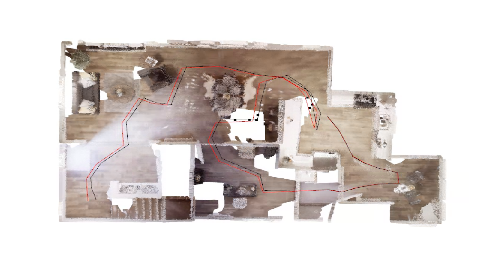
\includegraphics[width=0.47\linewidth]{image5.png}\hfill
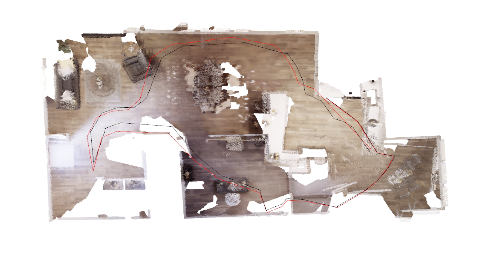
\includegraphics[width=0.47\linewidth]{image6.png}
\caption{Reference first-floor reconstruction results extracted from \texttt{HW2\_spec 2026.md}. The left and right examples use different data sizes (152 and 129, respectively); the red and black lines show the estimated and ground-truth trajectories.}
\label{fig:phase1-reference-results}
\end{figure}

\subsubsection{Phase 2: Second Floor of apartment\_0}
\begin{enumerate}
\item Control an agent in Habitat-Sim to navigate around the second floor of apartment\_0 and collect synchronized RGB images, depth images, and camera poses \cite{habitatsim2020,replica2019}.
\item Plan a route with useful spatial coverage and overlap between neighboring observations; document the route, frame spacing, and collection settings.
\item Run the same Standard Track reconstruction and evaluate the trajectory using Mean L2 Distance.
\item Measure and inspect quality factors, preserving values, settings, and links to relevant frames or pairs.
\item Compare Phase 2 with Phase 1 and discuss how coverage, viewpoint spacing, data quality, and algorithm parameters influenced reconstruction.
\end{enumerate}

\begin{figure}[htbp]
\centering
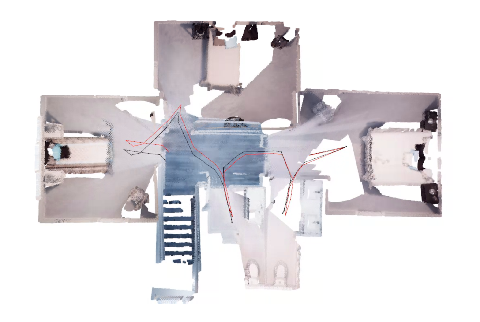
\includegraphics[width=0.78\linewidth]{image7.png}
\caption{Reference second-floor reconstruction result extracted from \texttt{HW2\_spec 2026.md} (data size 213). The red and black lines show the estimated and ground-truth trajectories.}
\label{fig:phase2-reference-result}
\end{figure}

\subsection{Bonus Track: My ICP Version (Optional Bonus)}
Implementing a custom ICP method is optional. For the Bonus Track, implement the method named \code{my_local_icp_algorithm}, including nearest-neighbor correspondence search and transformation estimation. Compare its result and runtime with the required Open3D version \cite{chen1992object,open3dglobal}. This is a bonus part and is not required for the base score.

% ============================================================
\section{Deliverables and Submission}
% ============================================================
\subsection{Submission Package}
Submit exactly \code{<student-id>_hw1.zip} to the designated submission platform. The zip root MUST have the following structure; do not add an extra enclosing directory:
\begin{lstlisting}
<student-id>_hw1.zip
|-- load.py
|-- reconstruct.py
|-- utils.py
|-- api.py
|-- ontology/
|   `-- hw1.ttl
|-- report.pdf
`-- README.md
\end{lstlisting}

The required source files are the files used by the submitted reconstruction and verification pipeline. If you implement the optional Bonus Track, include the implementation of \code{my_local_icp_algorithm} in the submitted source and identify it in \code{README.md}; the bonus code must not replace or break the required Open3D path. Experiment declaration Turtle files, generated diagnostics, and the Phase 2 capture directory are not required. Include the report. Do not include the large Replica environment archive or unrelated build artifacts.

\subsection{Report Contents}
The report MUST be a concise Portable Document Format (PDF) file written in English and include:
\begin{itemize}
\item Discuss the results of every required pipeline step and the data-verification workflow, and share your findings;
\item A concise explanation of the issues encountered during implementation, the solutions used to address them, and the justification for those choices;
\item Reconstruction screenshots for both phases, with the ceiling removed when needed, the estimated trajectory in red, and the GT trajectory in black;
\item A comparison table containing Mean L2 Distance, evaluated frame count, total execution time, and tested hyperparameters;
\item The data-quality measurements, settings, source links, failure cases, and a discussion of how the evidence relates to reconstruction;
\item Answers to the questions in the Assessment and Grading section;
\item If the Bonus Track is attempted, a comparison of the custom ICP and Open3D results, runtime, and implementation choices.
\end{itemize}

\subsection{Submission Rules}
\begin{itemize}
\item \textbf{Submission deadline:} the date and time announced for HW1 are the official deadline. The submission timestamp is determined by the designated submission platform.
\item A wrong submission format or an extra top-level directory leads to a $-10$ point penalty.
\item A late submission leads to a $-20$ point penalty per day.
\item Plagiarism is strictly prohibited, including code or reports copied from other students or public repositories. Any confirmed plagiarism results in a zero score without room for objection.
\item A report not written in English receives a score of zero.
\end{itemize}

% ============================================================
\section{Assessment and Grading}
% ============================================================
The base score is 100 points: the submitted program implementation accounts for 30\%, and the report accounts for the remaining 70\%. Implementing a custom ICP is optional and can earn an additional bonus.

\subsection{Program Implementation (30\%)}
The submitted program is assessed based on the required Open3D reconstruction, data collection and verification workflow, reproducibility, and source organization. The Standard Track is the complete base implementation. The optional Bonus Track is assessed from the submitted custom ICP implementation, its reconstruction result, and its documented comparison with the Open3D version.

\subsection{Report (70\%)}
\begin{center}
\begin{tabular}{L{0.58\linewidth} r}
\toprule
\textbf{Criterion} & \textbf{Weight} \\
\midrule
Pipeline implementation and data verification & 40\% \\
Results, Mean L2 evaluation, visualizations, and discussion & 20\% \\
Questions and technical analysis & 10\% \\
\midrule
Report total & 70\% \\
\midrule
Program implementation (submitted code) & 30\% \\
Base score total & 100\% \\
Optional custom ICP bonus & +20\% \\
\bottomrule
\end{tabular}
\end{center}

\subsection{Questions}
Answer the following questions in the report:
\begin{enumerate}
\item What happens if you perform ICP without global registration (RANSAC)? Why?
\item Describe any choices used to improve ICP stability, such as voxel size, correspondence thresholds, or robust losses.
\item How did the observed data-quality factors and collection choices affect the reconstruction and its Mean L2 Distance?
\end{enumerate}

\subsection{Optional Bonus (+20\%)}
\textbf{Custom own ICP:} Successful implementation of \code{my_local_icp_algorithm} with a meaningful comparison and performance comparable to the Open3D version.

This is an optional bonus part.

Students who submit only the Standard Track are not penalized.

% ============================================================
\printbibliography
\end{document}